\documentclass{article}
\usepackage{graphicx} %package to manage images
\graphicspath{ {./figures/} }
\usepackage{hyperref}
\usepackage{caption}
\usepackage[font=scriptsize]{subcaption}
\captionsetup[figure]{labelsep=none}
\captionsetup[table]{labelsep=none}
\usepackage{bbm}
\usepackage{amsmath}
\usepackage{import}
\usepackage{array}
\usepackage{booktabs}
\usepackage{afterpage}
\usepackage{floatrow}
\usepackage{pdflscape}
\usepackage{soul}
\usepackage{float}
\usepackage{adjustbox}
\usepackage{longtable}

\begin{document}


\maketitle

\section{main result}

\begin{figure}[H]
    \centering
    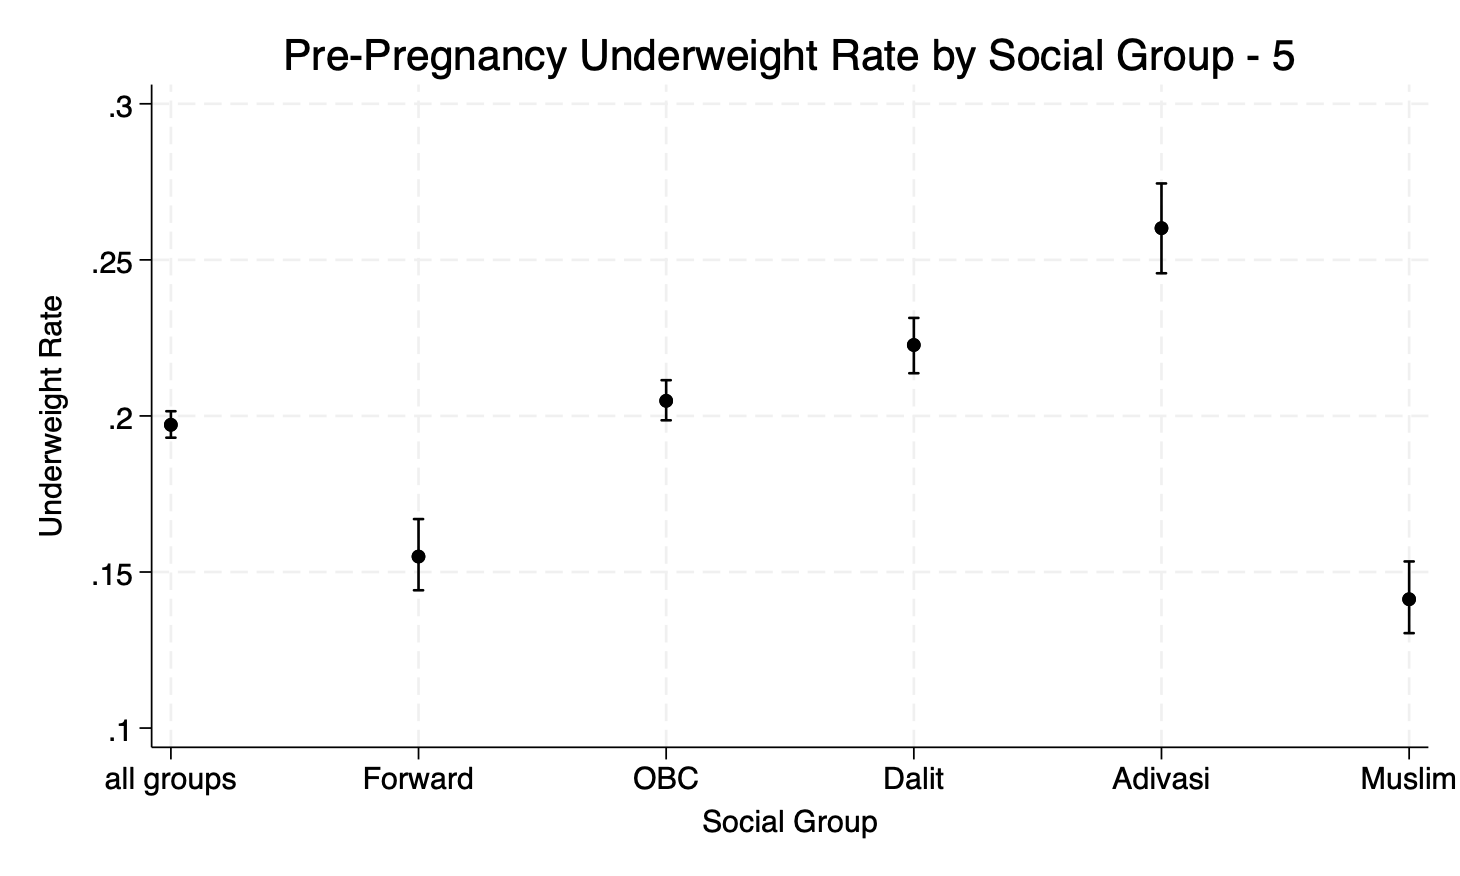
\includegraphics[width=\textwidth]{figures/bootstrapped_underweight_by_group_5.png}
\end{figure}


\section{kitagawa decomposition by parity + birth space}

% reweighting variables
% \begin{enumerate}
%     \item \textbf{Age bin}: 5--19, 20--24, 25--29, 30--34, 35--49.
%     \item \textbf{Wealth}: bottom half, upper half.
%     \item \textbf{Parity + birth spacing}: (as shown in the columns below).
%     \item \textbf{Contraceptive user}.
%     \item \textbf{Has boy child}.
%     \item \textbf{Urban/rural}.
%     \item \textbf{Less education}.
% \end{enumerate}


% groups with more than 3\% of pregnant women dropped
%  - Muslim parity 3 with birth spacing 2-3 yrs: 4.58\%

\begin{table}[H]
    \centering
    \footnotesize % shrink text
    \caption{: Dalit fwd decomposition}
    \label{tab:sumstat}
    \adjustbox{width=\textwidth}{\begin{tabular}{l*{12}{c}}
\toprule
            &\multicolumn{1}{c}{p1}&\multicolumn{1}{c}{p2 \textless2yrs}&\multicolumn{1}{c}{p2 2-3yrs}&\multicolumn{1}{c}{p3 \textless3yrs}&\multicolumn{1}{c}{p3 <2yrs}&\multicolumn{1}{c}{p3 2-3yrs}&\multicolumn{1}{c}{p3 >3yrs}&\multicolumn{1}{c}{p4+ <2yrs}&\multicolumn{1}{c}{p4+ 2-3yrs}&\multicolumn{1}{c}{p4+ >3yrs}&\multicolumn{1}{c}{total}&\multicolumn{1}{c}{pct}\\
\midrule
\midrule
Prop. preg (Fwd)&        0.49&        0.13&        0.07&        0.17&        0.04&        0.02&        0.04&        0.02&        0.01&        0.02&            &            \\
Avg pre-preg underweight (Fwd)&       15.72&       20.19&       15.73&       10.78&       18.07&       18.16&       10.97&       22.07&       13.00&       13.47&       11.30&            \\
Prop. preg (Dalit)&        0.41&        0.16&        0.06&        0.10&        0.08&        0.03&        0.04&        0.06&        0.03&        0.03&            &            \\
Avg pre-preg underweight (Dalit)&       22.71&       24.95&       23.59&       14.42&       25.08&       22.67&       17.67&       25.09&       20.92&       20.23&       14.86&            \\
Difference in underweight (Dalit-Forward)&        6.99&        4.75&        7.87&        3.64&        7.01&        4.51&        6.69&        3.02&        7.92&        6.76&        3.56&            \\
Within group difference&        3.13&        0.70&        0.51&        0.49&        0.41&        0.12&        0.27&        0.13&        0.14&        0.15&        4.34&      121.79\\
Between group difference&       -1.53&        0.83&       -0.07&       -0.85&        0.75&        0.22&        0.11&        0.80&        0.26&        0.20&       -0.78&      -21.79\\
\bottomrule
\end{tabular}
}
\end{table}

\begin{table}[H]
    \centering
    \footnotesize % shrink text
    \caption{: Adivasi fwd decomposition}
    \label{tab:sumstat}
    \adjustbox{width=\textwidth}{\begin{tabular}{l*{12}{c}}
\toprule
            &\multicolumn{1}{c}{p1}&\multicolumn{1}{c}{p2 \textless2yrs}&\multicolumn{1}{c}{p2 2-3yrs}&\multicolumn{1}{c}{p3 \textless3yrs}&\multicolumn{1}{c}{p3 <2yrs}&\multicolumn{1}{c}{p3 2-3yrs}&\multicolumn{1}{c}{p3 >3yrs}&\multicolumn{1}{c}{p4+ <2yrs}&\multicolumn{1}{c}{p4+ 2-3yrs}&\multicolumn{1}{c}{p4+ >3yrs}&\multicolumn{1}{c}{total}&\multicolumn{1}{c}{pct}\\
\midrule
\midrule
Prop. preg (Fwd)&        0.49&        0.13&        0.07&        0.17&        0.04&        0.02&        0.04&        0.02&        0.01&        0.02&            &            \\
Avg pre-preg underweight (Fwd)&       15.72&       20.19&       15.73&       10.78&       18.07&       18.16&       10.97&       22.07&       13.00&       13.47&       11.30&            \\
Prop. preg (Adivasi)&        0.39&        0.13&        0.07&        0.12&        0.06&        0.03&        0.07&        0.06&        0.03&        0.03&            &            \\
Avg pre-preg underweight (Adivasi)&       28.18&       30.00&       27.13&       16.67&       30.11&       31.57&       18.37&       30.18&       29.60&       22.19&       16.93&            \\
Difference in underweight (Adivasi-Forward)&       12.46&        9.81&       11.40&        5.88&       12.05&       13.42&        7.39&        8.11&       16.59&        8.71&        5.63&            \\
Within group difference&        5.47&        1.26&        0.81&        0.85&        0.62&        0.37&        0.38&        0.35&        0.31&        0.22&        7.54&      134.07\\
Between group difference&       -2.12&        0.03&        0.17&       -0.62&        0.48&        0.30&        0.44&        0.97&        0.35&        0.30&       -1.92&      -34.07\\
\bottomrule
\end{tabular}
}
\end{table}



\begin{table}[H]
    \centering
    \footnotesize % shrink text
    \caption{: Muslim fwd decomposition}
    \label{tab:sumstat}
    \adjustbox{width=\textwidth}{\begin{tabular}{l*{12}{c}}
\toprule
            &\multicolumn{1}{c}{p1}&\multicolumn{1}{c}{p2 <2yrs}&\multicolumn{1}{c}{p2 2-3yrs}&\multicolumn{1}{c}{p3 >3yrs}&\multicolumn{1}{c}{p3 <2yrs}&\multicolumn{1}{c}{p3 2-3yrs}&\multicolumn{1}{c}{p3 >3yrs}&\multicolumn{1}{c}{p4+ <2yrs}&\multicolumn{1}{c}{p4+ 2-3yrs}&\multicolumn{1}{c}{p4+ >3yrs}&\multicolumn{1}{c}{total}&\multicolumn{1}{c}{pct}\\
\midrule
\midrule
Prop. pregnant women (Fwd)&        0.49&        0.13&        0.07&        0.17&        0.04&        0.02&        0.04&        0.02&        0.01&        0.02&            &            \\
Avg pre-pregnancy underweight (Fwd)&       15.72&       20.19&       15.73&       10.78&       18.07&       18.16&       10.97&       22.07&       13.00&       13.47&       11.30&            \\
Prop. pregnant women (Muslim)&        0.38&        0.09&        0.05&        0.12&        0.06&        0.04&        0.10&        0.08&        0.03&        0.05&            &            \\
Avg pre-pregnancy underweight (Muslim)&       15.32&       18.02&       17.55&        7.93&       17.47&       16.44&        7.03&       15.64&       15.22&       11.65&        8.36&            \\
Difference in underweight (Muslim-Forward)&       -0.40&       -2.18&        1.82&       -2.85&       -0.60&       -1.72&       -3.94&       -6.43&        2.21&       -1.83&       -2.94&            \\
Within group difference&       -0.17&       -0.24&        0.11&       -0.41&       -0.03&       -0.05&       -0.26&       -0.33&        0.04&       -0.07&       -0.31&       10.56\\
Between group difference&       -1.73&       -0.63&       -0.27&       -0.42&        0.29&        0.32&        0.53&        1.03&        0.28&        0.47&       -2.63&       89.44\\
\bottomrule
\end{tabular}
}
\end{table}

\begin{table}[H]
    \centering
    \footnotesize % shrink text
    \caption{: OBC fwd decomposition}
    \label{tab:sumstat}
    \adjustbox{width=\textwidth}{\begin{tabular}{l*{12}{c}}
\toprule
            &\multicolumn{1}{c}{p1}&\multicolumn{1}{c}{p2 \textless2yrs}&\multicolumn{1}{c}{p2 2-3yrs}&\multicolumn{1}{c}{p2 \textgreater3yrs}&\multicolumn{1}{c}{p3 \textless2yrs}&\multicolumn{1}{c}{p3 2-3yrs}&\multicolumn{1}{c}{p3 \textgreater3yrs}&\multicolumn{1}{c}{p4+ \textless2yrs}&\multicolumn{1}{c}{p4+ 2-3yrs}&\multicolumn{1}{c}{p4+ \textgreater3yrs}&\multicolumn{1}{c}{total}&\multicolumn{1}{c}{pct}\\
\midrule
\midrule
Prop. preg (Fwd)&        0.49&        0.13&        0.07&        0.17&        0.04&        0.02&        0.04&        0.02&        0.01&        0.02&            &            \\
Avg pre-preg underweight (Fwd)&       15.72&       20.19&       15.73&       10.78&       18.07&       18.16&       10.97&       22.07&       13.00&       13.47&       15.54&            \\
Prop. preg (OBC)&        0.43&        0.16&        0.07&        0.12&        0.07&        0.03&        0.04&        0.04&        0.02&        0.02&            &            \\
Avg pre-preg underweight (OBC)&       21.08&       23.74&       19.92&       12.49&       23.73&       22.79&       12.96&       23.70&       24.82&       17.30&       20.37&            \\
Difference in underweight (OBC-Forward)&        5.36&        3.55&        4.20&        1.70&        5.66&        4.64&        1.99&        1.63&       11.82&        3.82&        4.83&            \\
Within group difference&        2.46&        0.50&        0.29&        0.24&        0.30&        0.12&        0.08&        0.05&        0.17&        0.07&        4.30&       88.94\\
Between group difference&       -1.01&        0.62&        0.06&       -0.56&        0.52&        0.17&        0.08&        0.41&        0.15&        0.08&        0.53&       11.06\\
\bottomrule
\end{tabular}
}
\end{table}

\section{kitagawa decomposition by birth space}

% reweighting variables
% \begin{enumerate}
%     \item \textbf{Age bin}: 5--19, 20--24, 25--29, 30--34, 35--49.
%     \item \textbf{Wealth}: 4 quartiles.
%     \item \textbf{Parity + birth spacing}: (as shown in the columns below).
%     \item \textbf{Contraceptive user}.
%     \item \textbf{Has boy child}.
%     \item \textbf{Urban/rural}.
%     \item \textbf{Less education}.
% \end{enumerate}


% groups with more than 3\% of pregnant women dropped
%  - Forward with birth spacing 2-3 years: 3.58\%
%  - Dalit with birth spacing 2-3 years: 3.36\%
%  - Muslim with birth spacing 2-3 years: 5.29\%

\begin{table}[H]
    \centering
    \footnotesize % shrink text
    \caption{: Dalit fwd decomposition}
    \label{tab:sumstat}
    \adjustbox{width=\textwidth}{\begin{tabular}{l*{5}{c}}
\toprule
            &\multicolumn{1}{c}{under 2 yrs}&\multicolumn{1}{c}{2-3 years}&\multicolumn{1}{c}{over 3 years}&\multicolumn{1}{c}{Total}&\multicolumn{1}{c}{Percent}\\
\midrule
\midrule
Prop. pregnant women (Fwd)&        0.19&        0.10&        0.22&            &            \\
Avg pre-pregnancy underweight (Fwd)&       19.89&       13.62&       11.20&        7.66&            \\
Prop. pregnant women (Dalit)&        0.30&        0.12&        0.17&            &            \\
Avg pre-pregnancy underweight (Dalit)&       24.63&       22.33&       15.64&       12.76&            \\
Difference in underweight (Dalit-Forward)&        4.73&        8.71&        4.44&        5.10&            \\
Within parity difference (rate)&        1.17&        0.96&        0.87&        2.99&       58.70\\
Between parity difference (compositional)&        2.35&        0.40&       -0.64&        2.11&       41.30\\
\bottomrule
\end{tabular}
}
\end{table}

\begin{table}[H]
    \centering
    \footnotesize % shrink text
    \caption{: Adivasi fwd decomposition}
    \label{tab:sumstat}
    \adjustbox{width=\textwidth}{\begin{tabular}{l*{5}{c}}
\toprule
            &\multicolumn{1}{c}{under 2 yrs}&\multicolumn{1}{c}{2-3 years}&\multicolumn{1}{c}{over 3 years}&\multicolumn{1}{c}{Total}&\multicolumn{1}{c}{Percent}\\
\midrule
\midrule
Prop. pregnant women (Fwd)&        0.19&        0.10&        0.22&            &            \\
Avg pre-pregnancy underweight (Fwd)&       20.00&       15.98&       11.02&        7.88&            \\
Prop. pregnant women (Adivasi)&        0.25&        0.14&        0.22&            &            \\
Avg pre-pregnancy underweight (Adivasi)&       30.07&       28.73&       18.01&       15.45&            \\
Difference in underweight (Adivasi-Forward)&       10.07&       12.76&        6.98&        7.58&            \\
Within parity difference (rate)&        2.24&        1.49&        1.54&        5.28&       69.67\\
Between parity difference (compositional)&        1.46&        0.82&        0.02&        2.30&       30.33\\
\bottomrule
\end{tabular}
}
\end{table}


\begin{table}[H]
    \centering
    \footnotesize % shrink text
    \caption{: Muslim fwd decomposition}
    \label{tab:sumstat}
    \adjustbox{width=\textwidth}{\begin{tabular}{l*{5}{c}}
\toprule
            &\multicolumn{1}{c}{under 2 yrs}&\multicolumn{1}{c}{2-3 years}&\multicolumn{1}{c}{over 3 years}&\multicolumn{1}{c}{Total}&\multicolumn{1}{c}{Percent}\\
\midrule
\midrule
Prop. pregnant women (Fwd)&        0.38&        0.19&        0.43&            &            \\
Avg pre-pregnancy underweight (Fwd)&       20.84&       16.39&       11.69&       16.05&            \\
Prop. pregnant women (Muslim)&        0.37&        0.19&        0.44&            &            \\
Avg pre-pregnancy underweight (Muslim)&       17.39&       18.49&        9.10&       13.99&            \\
Difference in underweight (Muslim-Forward)&       -3.45&        2.09&       -2.59&       -2.06&            \\
Within parity difference (rate)&       -1.29&        0.40&       -1.12&       -2.01&       97.27\\
Between parity difference (compositional)&       -0.13&        0.01&        0.07&       -0.06&        2.73\\
\bottomrule
\end{tabular}
}
\end{table}

\begin{table}[H]
    \centering
    \footnotesize % shrink text
    \caption{: OBC fwd decomposition}
    \label{tab:sumstat}
    \adjustbox{width=\textwidth}{\begin{tabular}{l*{5}{c}}
\toprule
            &\multicolumn{1}{c}{under 2 yrs}&\multicolumn{1}{c}{2-3 years}&\multicolumn{1}{c}{over 3 years}&\multicolumn{1}{c}{Total}&\multicolumn{1}{c}{Percent}\\
\midrule
\midrule
Prop. pregnant women (Fwd)&        0.19&        0.10&        0.22&            &            \\
Avg pre-pregnancy underweight (Fwd)&       19.89&       13.62&       11.20&        7.66&            \\
Prop. pregnant women (OBC)&        0.27&        0.12&        0.18&            &            \\
Avg pre-pregnancy underweight (OBC)&       22.74&       20.39&       13.63&       10.95&            \\
Difference in underweight (OBC-Forward)&        2.84&        6.77&        2.43&        3.29&            \\
Within parity difference (rate)&        0.65&        0.73&        0.49&        1.88&       57.13\\
Between parity difference (compositional)&        1.52&        0.34&       -0.45&        1.41&       42.87\\
\bottomrule
\end{tabular}
}
\end{table}





\section{kitagawa decomposition by parity}

% reweighting variables
% \begin{enumerate}
%     \item \textbf{Age bin}: 5--19, 20--24, 25--29, 30--34, 35--49.
%     \item \textbf{Wealth}: 4 quartiles.
%     \item \textbf{Parity + birth spacing}: (as shown in the columns below).
%     \item \textbf{Contraceptive user}.
%     \item \textbf{Has boy child}.
%     \item \textbf{Urban/rural}.
%     \item \textbf{Less education}.
% \end{enumerate}


\begin{table}[H]
    \centering
    \footnotesize % shrink text
    \caption{: Dalit fwd decomposition}
    \label{tab:sumstat}
    \adjustbox{width=\textwidth}{\begin{tabular}{l*{6}{c}}
\toprule
            &\multicolumn{1}{c}{mtitles1}&\multicolumn{1}{c}{parity2}&\multicolumn{1}{c}{parity3}&\multicolumn{1}{c}{parity4}&\multicolumn{1}{c}{total}&\multicolumn{1}{c}{pct}\\
\midrule
\midrule
Prop. preg (Fwd)&        0.49&        0.36&        0.10&        0.05&            &            \\
Avg pre-preg underweight (Fwd)&       15.72&       15.02&       15.44&       17.47&       15.53&            \\
Prop. preg (Dalit)&        0.41&        0.33&        0.15&        0.11&            &            \\
Avg pre-preg underweight (Dalit)&       22.71&       21.48&       22.43&       22.90&       22.29&            \\
Difference in underweight (Dalit-Forward)&        6.99&        6.46&        6.99&        5.43&        6.76&            \\
Within group difference&        3.13&        2.23&        0.87&        0.45&        6.68&       98.84\\
Between group difference&       -1.53&       -0.63&        1.01&        1.24&        0.08&        1.16\\
\bottomrule
\end{tabular}
}
\end{table}

\begin{table}[H]
    \centering
    \footnotesize % shrink text
    \caption{: Adivasi fwd decomposition}
    \label{tab:sumstat}
    \adjustbox{width=\textwidth}{\begin{tabular}{l*{6}{c}}
\toprule
            &\multicolumn{1}{c}{mtitles1}&\multicolumn{1}{c}{parity2}&\multicolumn{1}{c}{parity3}&\multicolumn{1}{c}{parity4}&\multicolumn{1}{c}{total}&\multicolumn{1}{c}{pct}\\
\midrule
\midrule
Prop. preg (Fwd)&        0.49&        0.36&        0.10&        0.05&            &            \\
Avg pre-preg underweight (Fwd)&       15.72&       15.02&       15.44&       17.47&       15.53&            \\
Prop. preg (Adivasi)&        0.39&        0.33&        0.16&        0.12&            &            \\
Avg pre-preg underweight (Adivasi)&       28.18&       24.35&       25.59&       27.85&       26.47&            \\
Difference in underweight (Adivasi-Forward)&       12.46&        9.33&       10.14&       10.37&       10.94&            \\
Within group difference&        5.47&        3.21&        1.31&        0.90&       10.90&       99.61\\
Between group difference&       -2.12&       -0.71&        1.27&        1.59&        0.04&        0.39\\
\bottomrule
\end{tabular}
}
\end{table}



\begin{table}[H]
    \centering
    \footnotesize % shrink text
    \caption{: Muslim fwd decomposition}
    \label{tab:sumstat}
    \adjustbox{width=\textwidth}{\begin{tabular}{l*{6}{c}}
\toprule
            &\multicolumn{1}{c}{parity 1}&\multicolumn{1}{c}{parity 2}&\multicolumn{1}{c}{parity 3}&\multicolumn{1}{c}{parity 4+}&\multicolumn{1}{c}{Total}&\multicolumn{1}{c}{Percent}\\
\midrule
\midrule
Prop. preg (Fwd)&        0.49&        0.36&        0.10&        0.05&            &            \\
Avg pre-preg underweight (Fwd)&       15.72&       15.02&       15.44&       17.47&       15.53&            \\
Prop. preg (Muslim)&        0.38&        0.27&        0.19&        0.16&            &            \\
Avg pre-preg underweight (Muslim)&       15.32&       13.30&       12.04&       14.22&       13.97&            \\
Difference in underweight (Muslim-Forward)&       -0.40&       -1.72&       -3.40&       -3.25&       -1.56&            \\
Within group difference&       -0.17&       -0.54&       -0.50&       -0.35&       -1.56&       99.93\\
Between group difference&       -1.73&       -1.34&        1.29&        1.78&       -0.00&        0.07\\
\bottomrule
\end{tabular}
}
\end{table}

\begin{table}[H]
    \centering
    \footnotesize % shrink text
    \caption{: OBC fwd decomposition}
    \label{tab:sumstat}
    \adjustbox{width=\textwidth}{\begin{tabular}{l*{6}{c}}
\toprule
            &\multicolumn{1}{c}{mtitles1}&\multicolumn{1}{c}{parity2}&\multicolumn{1}{c}{parity3}&\multicolumn{1}{c}{parity4}&\multicolumn{1}{c}{total}&\multicolumn{1}{c}{pct}\\
\midrule
\midrule
Prop. preg (Fwd)&        0.49&        0.36&        0.10&        0.05&            &            \\
Avg pre-preg underweight (Fwd)&       15.72&       15.02&       15.44&       17.47&       15.53&            \\
Prop. preg (OBC)&        0.43&        0.35&        0.14&        0.08&            &            \\
Avg pre-preg underweight (OBC)&       21.08&       19.09&       20.21&       22.23&       20.37&            \\
Difference in underweight (OBC-Forward)&        5.36&        4.07&        4.77&        4.76&        4.84&            \\
Within group difference&        2.46&        1.44&        0.57&        0.32&        4.79&       99.07\\
Between group difference&       -1.01&       -0.28&        0.71&        0.62&        0.05&        0.93\\
\bottomrule
\end{tabular}
}
\end{table}


\section{kitagawa decomposition by wealth}

% reweighting variables
% \begin{enumerate}
%     \item \textbf{Age bin}: 5--19, 20--24, 25--29, 30--34, 35--49.
%     \item \textbf{Wealth}: 4 quartiles.
%     \item \textbf{Parity + birth spacing}: (as shown in the columns below).
%     \item \textbf{Contraceptive user}.
%     \item \textbf{Has boy child}.
%     \item \textbf{Urban/rural}.
%     \item \textbf{Less education}.
% \end{enumerate}


\begin{table}[H]
    \centering
    \footnotesize % shrink text
    \caption{: Dalit fwd decomposition}
    \label{tab:sumstat}
    \adjustbox{width=\textwidth}{\begin{tabular}{l*{6}{c}}
\toprule
            &\multicolumn{1}{c}{Wealth 1st Q}&\multicolumn{1}{c}{Wealth 2nd Q}&\multicolumn{1}{c}{Wealth 3rd Q}&\multicolumn{1}{c}{Wealth 4th Q}&\multicolumn{1}{c}{Total}&\multicolumn{1}{c}{Percent}\\
\midrule
\midrule
Prop. pregnant women (Fwd)&        0.11&        0.17&        0.27&        0.44&            &            \\
Avg pre-pregnancy underweight (Fwd)&       25.40&       23.42&       15.24&       11.06&       15.97&            \\
Prop. pregnant women (Dalit)&        0.34&        0.26&        0.24&        0.16&            &            \\
Avg pre-pregnancy underweight (Dalit)&       29.28&       22.28&       19.24&       13.04&       22.41&            \\
Difference in underweight (Dalit-Forward)&        3.88&       -1.14&        3.99&        1.98&        6.45&            \\
Within parity difference (rate)&        0.88&       -0.24&        1.02&        0.60&        2.26&       34.99\\
Between parity difference (compositional)&        6.15&        1.96&       -0.59&       -3.33&        4.19&       65.01\\
\bottomrule
\end{tabular}
}
\end{table}

\begin{table}[H]
    \centering
    \footnotesize % shrink text
    \caption{: Adivasi fwd decomposition}
    \label{tab:sumstat}
    \adjustbox{width=\textwidth}{\begin{tabular}{l*{6}{c}}
\toprule
            &\multicolumn{1}{c}{Wealth 1st Q}&\multicolumn{1}{c}{Wealth 2nd Q}&\multicolumn{1}{c}{Wealth 3rd Q}&\multicolumn{1}{c}{Wealth 4th Q}&\multicolumn{1}{c}{Total}&\multicolumn{1}{c}{Percent}\\
\midrule
\midrule
Prop. pregnant women (Fwd)&        0.11&        0.17&        0.27&        0.44&            &            \\
Avg pre-pregnancy underweight (Fwd)&       27.24&       23.80&       15.34&       11.01&       16.24&            \\
Prop. pregnant women (Adivasi)&        0.50&        0.25&        0.16&        0.09&            &            \\
Avg pre-pregnancy underweight (Adivasi)&       30.61&       27.54&       20.37&       10.81&       26.34&            \\
Difference in underweight (Adivasi-Forward)&        3.37&        3.73&        5.03&       -0.19&       10.10&            \\
Within parity difference (rate)&        1.03&        0.78&        1.09&       -0.05&        2.86&       28.29\\
Between parity difference (compositional)&       11.11&        1.91&       -2.00&       -3.78&        7.24&       71.71\\
\bottomrule
\end{tabular}
}
\end{table}



\begin{table}[H]
    \centering
    \footnotesize % shrink text
    \caption{: Muslim fwd decomposition}
    \label{tab:sumstat}
    \adjustbox{width=\textwidth}{\begin{tabular}{l*{6}{c}}
\toprule
            &\multicolumn{1}{c}{Wealth 1st Q}&\multicolumn{1}{c}{Wealth 2nd Q}&\multicolumn{1}{c}{Wealth 3rd Q}&\multicolumn{1}{c}{Wealth 4th Q}&\multicolumn{1}{c}{Total}&\multicolumn{1}{c}{Percent}\\
\midrule
\midrule
Prop. preg (Fwd)&        0.11&        0.17&        0.27&        0.44&            &            \\
Avg pre-preg underweight (Fwd)&       25.47&       23.29&       13.97&       10.92&       15.54&            \\
Prop. preg (Muslim)&        0.26&        0.23&        0.25&        0.27&            &            \\
Avg pre-preg underweight (Muslim)&       20.39&       15.20&       11.96&        8.87&       14.05&            \\
Difference in underweight (Muslim-Forward)&       -5.08&       -8.09&       -2.01&       -2.05&       -1.49&            \\
Within group difference&       -0.95&       -1.61&       -0.52&       -0.73&       -3.81&      255.69\\
Between group difference&        3.33&        1.03&       -0.33&       -1.72&        2.32&     -155.69\\
\bottomrule
\end{tabular}
}
\end{table}

\begin{table}[H]
    \centering
    \footnotesize % shrink text
    \caption{: OBC fwd decomposition}
    \label{tab:sumstat}
    \adjustbox{width=\textwidth}{\begin{tabular}{l*{6}{c}}
\toprule
            &\multicolumn{1}{c}{mtitles1}&\multicolumn{1}{c}{wealth2}&\multicolumn{1}{c}{wealth3}&\multicolumn{1}{c}{wealth4}&\multicolumn{1}{c}{total}&\multicolumn{1}{c}{pct}\\
\midrule
\midrule
Prop. preg (Fwd)&        0.11&        0.17&        0.27&        0.44&            &            \\
Avg pre-preg underweight (Fwd)&       25.47&       23.29&       13.97&       10.92&       15.54&            \\
Prop. preg (OBC)&        0.22&        0.25&        0.26&        0.27&            &            \\
Avg pre-preg underweight (OBC)&       29.88&       23.91&       18.35&       11.64&       20.45&            \\
Difference in underweight (OBC-Forward)&        4.41&        0.62&        4.38&        0.72&        4.91&            \\
Within group difference&        0.74&        0.13&        1.17&        0.26&        2.29&       46.74\\
Between group difference&        3.01&        1.72&       -0.22&       -1.90&        2.61&       53.26\\
\bottomrule
\end{tabular}
}
\end{table}








\end{document}


